\pagebreak
\chapter{Skripte}
In diesem Kapitel werden die Skripte des Spieles als Code Blöcke dargestellt und erklärt. 

\section{Münzen Skript}
Das Münzen Skript ist dafür verantwortlich, dass die Münzen einsammelbar sind. 
% C#
\begin{lstlisting}[language=CSharp,caption={Coin Klasse.},label=code:coin]
    public class Coin : MonoBehaviour
    {
        private void OnTriggerEnter(Collider other)
        {
            if (other.gameObject == player)
            {
                float distance = Vector3.Distance(transform.position, player.transform.position);
                
                if (distance <= collectionRange)
                {
                    coinCounterText.text = (Int32.Parse(coinCounterText.text) + 1).ToString();
                    
                    Destroy(gameObject);
                }
            }
        }
    }
\end{lstlisting}   

Die Funktion der \verb+Coin+ Klasse ist sehr simpel. Zuerst wird geschaut ob es eine Collision mit einem anderem Game-Objekt gegeben hat. Wenn dieses andere Game-Objekt der Player war, wird noch die Distanz zu dem Player geprüft. Falls die Distanz innerhalb des Aufsammelradius ist, wird der \verb+coinCounterText+ von dem User Interface hochgezählt und die Münze zerstört.


\pagebreak
\section{Player Skripte}
Der Code für den Player unterteilt sich in zwei verschiedene Skripte. Einerseits gibt es die \verb+Player+ Klasse die für die Lebenspunkte des Spielers verantwortlich ist. Andererseits gibt es das \verb+PlayerMovement+ Skript, welches für die Kontrolle über den Charakter verantwortlich ist. \\

\subsection{Player Klasse}
% C#
\begin{lstlisting}[language=CSharp,caption={Player Klasse.},label=code:player]
public class Player : MonoBehaviour{
    private void Start(){
        currentHealth = maxHealth;
        healthbar.SetMaxHealth(maxHealth);
        damageOverlay.gameObject.SetActive(false);
        gameOverScreen.SetActive(false);
    }

    public void TakeDamage(int damage){
        ShowDamageOverlay();
        currentHealth -= damage;
        healthbar.SetHealth(currentHealth);
        if (currentHealth <= 0){
            Time.timeScale = 0f;
            gameOverScreen.SetActive(true);
        }
    }
}
\end{lstlisting}

Die Player Klasse enthält alle Informationen und Funktionen der Lebenspunkte des Charakters. In der \verb+Start()+ Methode wird die Anzahl von Lebenspunkten der Lebensanzeige übegeben. Weiters gibt es noch eine \verb+TakeDamage()+ Methode. Diese kann mit einer bestimmten Anzahl an Schaden aufgerufen werden. Bei dem Aufruf dieser Methode wird der Schaden den derzeitigen Lebenspunkten abgezogen und der Lebensanzeige neu übergeben. Außerdem wird mit einer \bettergls{coroutine}{1} kurzzeitig das DamageOverlay angezeigt. Falls der Spieler keine Lebenspunkte mehr hat, wird der GameOverScreen angezeigt.

\pagebreak

\subsection{PlayerMovement Klasse}
Die \verb+PlayerMovement+ Klasse unterteilt sich in zwei wichtige Funktionen. Der Code der dem Spieler ermöglicht sich zu bewegen und die Funktion für das Springen.\\

% C#
\begin{lstlisting}[language=CSharp,caption={CharacterMovement der PlayerMovement Klasse.},label=code:charactermovement]
    void CharacterMovement() {
        rotation.y += Input.GetAxis("Mouse X");
        transform.eulerAngles = (Vector2)rotation * 3f;
        
        float moveX = Input.GetAxisRaw("Horizontal");
        float moveZ = Input.GetAxisRaw("Vertical");
    
        Vector3 direction = new Vector3(moveX, 0, moveZ);
        direction.Normalize();
        transform.Translate(direction * (speed * Time.deltaTime));
    }
\end{lstlisting}

Es gibt zwei Wege wie die Bewegung der Spielfigur gehandhabt werden kann. Entweder ist die Bewegung statisch, oder sie ist dynamisch wie es in dem Listing oberhalb dargestellt ist. Die Methode nimmt die horizontale Bewegung der Maus und berechnet sich in welche Richtung sich der Charakter bewegen muss.\\

% C#
\begin{lstlisting}[language=CSharp,caption={Jump \& DoubleJump der PlayerMovement Klasse.},label=code:player]
    if (IsGrounded()){
        hasDoubleJump = true;
        if (Input.GetKeyDown(KeyCode.Space))
        {
            rb.AddForce(Vector3.up * JumpHeight, ForceMode.Impulse);
            //jumpSound.Play();
        }
    } else if (Input.GetKeyDown(KeyCode.Space) && hasDoubleJump){
        hasDoubleJump = false;
        rb.AddForce(transform.up * doubleJumpHeight, ForceMode.Impulse);
    }
\end{lstlisting}

Bei dem Code für das Springen muss zuerst geschaut werden, ob der Player auf dem Boden steht. Sobald dann die Springen-Taste gedrückt wird, wird dem Rigidbody des Charakters eine \verb+Force+ also eine vertikale Kraft nach oben addiert. Die Funktion wird bei dem zweiten Drücken der Sprung-Taste in der Luft ausgeführt.

\pagebreak
\section{Enemy Skript}

Bei dem Enemy Skript wurde, anstatt eines einfachen \verb+Waypointfollower+ wie es bei den beweglichen Plattformen der Fall ist, Unitys eingebauter AI verwendet. Damit dieser funktioniert benötigt die Scene zwei Komponenten. Ein NavMesh für die Plattform auf der sich der Gegner bewegen soll und einen NavMeshAgent für das Game-Objekt des Gegners.

\begin{figure}[h]
    \centering
    \begin{minipage}[b]{0.5\textwidth}
        \centering
        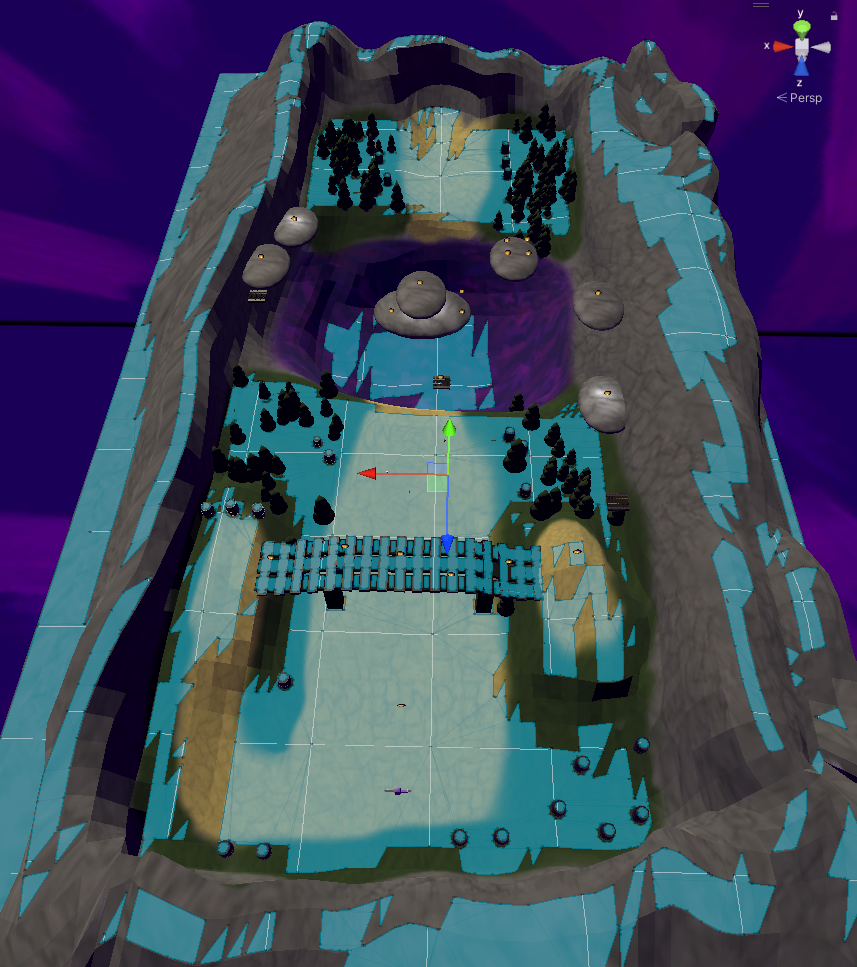
\includegraphics[width=\textwidth]{chapters/05/images/NavMesh.png}
        \caption{Das Nav Mesh in dem ersten Level des Prototypen.}
        \label{fig:SD01}
    \end{minipage}
    \hfill
    \begin{minipage}[b]{0.45\textwidth}
        \centering
        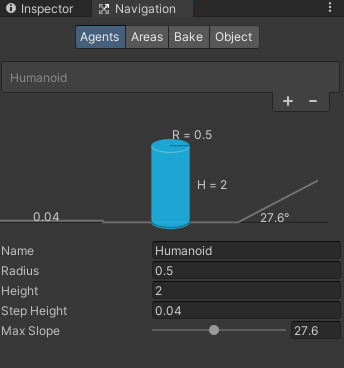
\includegraphics[width=\textwidth]{chapters/05/images/Agent.png}
        \caption{Der Agent für der Gegner.}
        \label{fig:PE0SD022}
    \end{minipage}
\end{figure}

In der linken Abbildung ist das Nav Mesh in Blau zu sehen. Dieses wird automatisch erstellt, wenn die Grundplattform ausgewählt wird und wie in der rechten Abbildung ein Agent erstellt wird. Bei dem dritten Tab kann das NavMesh \glqq baked\grqq \space werden. Die eingegebenen Zahlen bei dem Agent entscheiden die Oberflächen, über welche der NavMeshAgent sich hinfortbewegen kann. In dem Fall des ersten Levels wurden diese so eingestellt, dass der Agent vor und nach dem Abgrund eine größere Fläche hat um sich zu bewegen. 


\pagebreak
\subsection{Der Code des Enemy Skripts}
% C#
\begin{lstlisting}[language=CSharp,caption={EnemyController Klasse.},label=code:enemyController]
public class EnemyController : MonoBehaviour
{
    [SerializeField] private Transform movePositionTransform;

    private NavMeshAgent navMeshAgent;

    private void Awake()
    {
        navMeshAgent = GetComponent<NavMeshAgent>();
    }
    
    private void Update()
    {
        navMeshAgent.destination = movePositionTransform.position;
        Vector3 targetPostition = new Vector3( movePositionTransform.position.x, 
            this.transform.position.y, 
            movePositionTransform.position.z ) ;
        this.transform.LookAt( targetPostition ) ;
    }
}
\end{lstlisting}

\emph{\glqq Die NavMesh-Agentenkomponente verwaltet sowohl die Pfadfindung als auch die Bewegungssteuerung eines Spiel-Objekts. In den Skripten muss für eine einfache Navigation nur der gewünschte Zielpunkt festgelegt werden - der NavMesh-Agent kann alles Weitere von dort aus übernehemn.\grqq}~\cite[Unity NavMesh Dokumentation]{unitydocNavmesh} \\

Der EnemyController importiert den NavMeshAgent und eine Transform die als Ziel dient. Der für den Prototypen ausgewählte Zielpunkt ist der Player. Die Gegner werden dann automatisch Hindernissen ausweichen und versuchen an den Spieler heranzukommen. 

\pagebreak

\subsection{Die Deathzone}
Eine \bettergls{deathzone}{1} ist in der Videospiel Branche sehr bekannt. Unter Developern aber auch unter Spielern. Ohne einer Todeszone kann es leicht passieren, dass der Spieler aus der Map ins unendliche fällt. Zusätzlich kann mit dieser Restriktion verhindert werden das der Player über Wände klettert und damit Teile des Levels überspringt.\\

\begin{lstlisting}[language=CSharp,caption={DeathZone Klasse},label=code:deathzone]
public class DeathZone : MonoBehaviour
{
    public Player player;
    public int damageAmount;

    private Vector3 spawnPoint = new Vector3(9, -42, 168);
    void OnTriggerExit(Collider other)
    {
        other.transform.position = spawnPoint;
        player.TakeDamage(damageAmount);
    }
}
\end{lstlisting}

Die \verb+DeathZone+ Klasse benötigt nur das Game-Objekt des Spielers und eine Anzahl an Schaden. Wie in der Abbildung \ref{SD02} gezeigt wird, ist die Deathzone des Prototypen ein Quader. Dieser umfässt das komplette Level. Wenn der Player diese Zone verlässt, dann wird in \verb+OnTriggerExit+ das Game-Objekt wieder zurück an die Spawn Position gesetzt und dem Player wird Schaden hinzugefügt.

\begin{figure}[H]
    \centering
    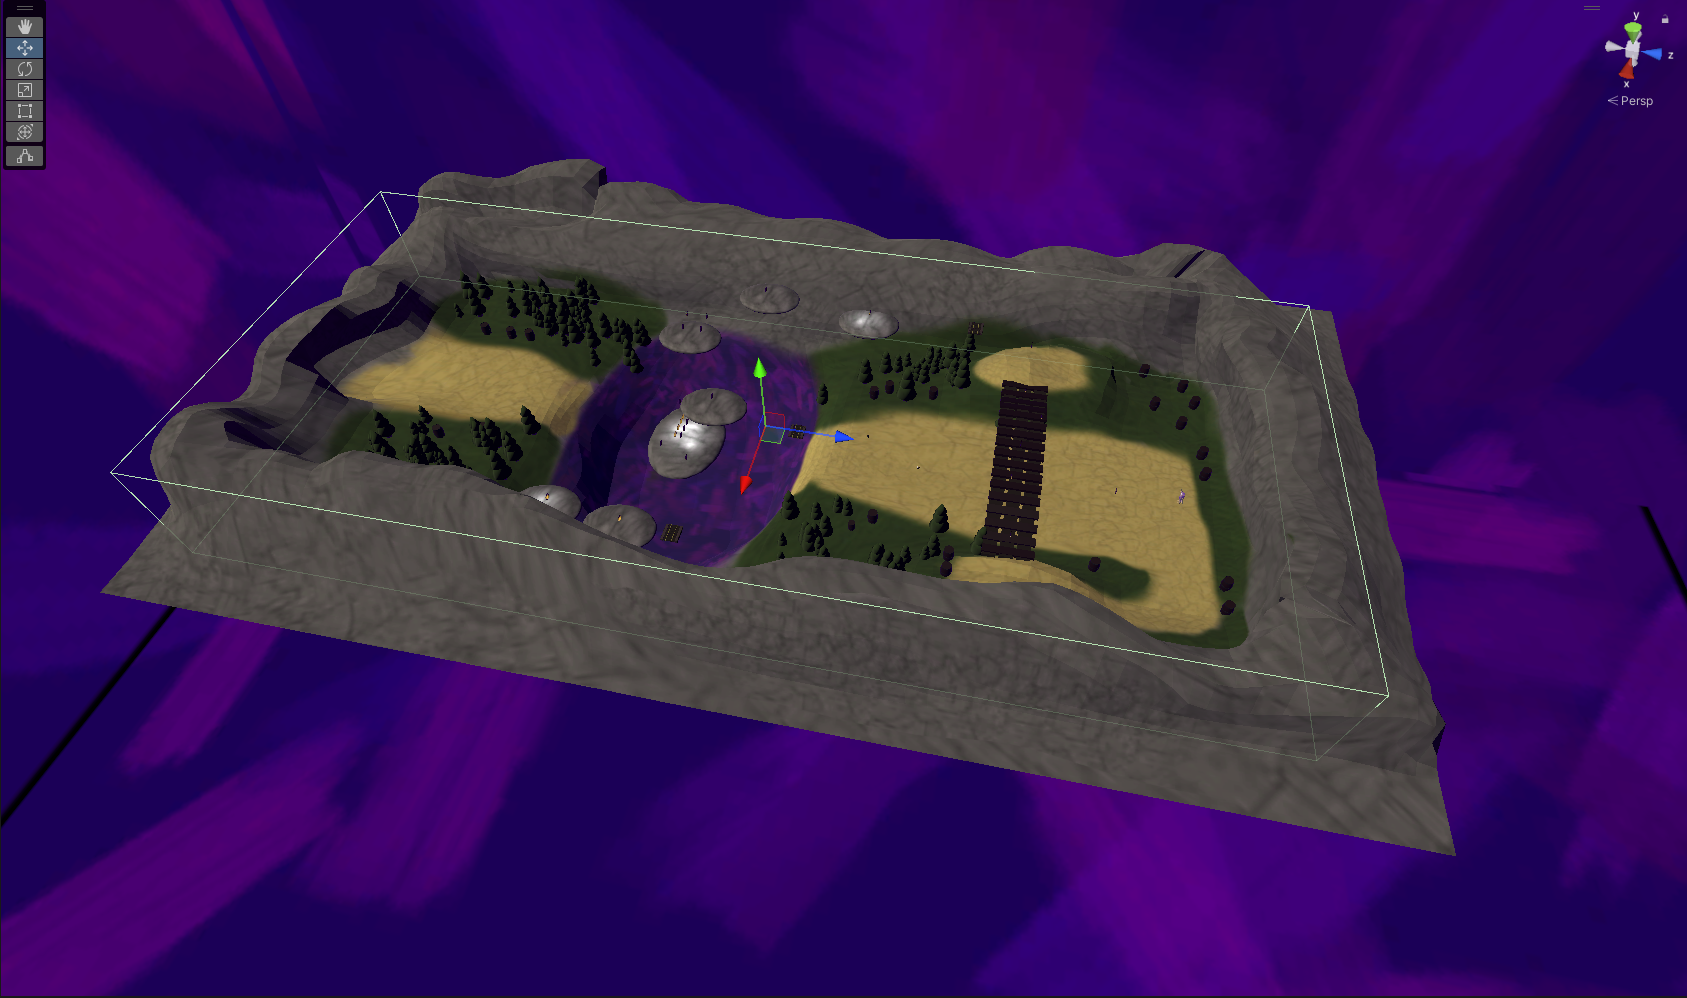
\includegraphics[width=0.8\textwidth]{chapters/05/images/DeathZone.png}
    \caption{Die DeathZone in dem Prototypen.}
    \label{SD02}
\end{figure}
\pagebreak


\subsection{WayPointFollower Skript}

\begin{lstlisting}[language=CSharp,caption={FixedUpdate der WayPointFollower Klasse.},label=code:mainmenu]
public class WaypointFollower : MonoBehaviour
{
  GameObject[] waypoints;
  int direction = 1; // 1 for forward, -1 for backward

  void FixedUpdate()
  {
      if (Vector3.Distance(transform.position, waypoints[currentWaypointIndex].transform.position) < .1f)
      {
          currentWaypointIndex += direction;

          if (currentWaypointIndex >= waypoints.Length || currentWaypointIndex < 0)
          {
              direction *= -1; // Reverse the direction when reaching the end or start
              currentWaypointIndex += direction * 2; // Move two steps in the opposite direction
          }
      }

      transform.position = Vector3.MoveTowards(transform.position, waypoints[currentWaypointIndex].transform.position, speed * Time.deltaTime);
  }
}
\end{lstlisting}

In dem oberhalb abgebildeten Listing ist ein Ausschnitt der \verb+WayPointFollower+ Klasse dargestellt. Die in Unity erstellten Wegpunkte werden in das GameObjekt Array gespeichert. Mittels dem \bettergls{index}{1} und der \verb+direction+ Variable wird durch dieses Array durch-\bettergls{iteriert}{2}. Wenn der Index außerhalb des Arrays von Wegpunkten angekommen ist, dann wird die \verb+direction+ umgedreht. Für die eigentliche Bewegung der Plattform ist die Methode \verb+Vector3.MoveTowards()+ verantwortlich. In dieser wird die aktuelle Position, die Position des Ziels und eine Entfernung übergeben.


\pagebreak

\subsection{StickyPlatform Skript}

\begin{lstlisting}[language=CSharp,caption={StickyPlatform Klasse.},label=code:mainmenu]
  public class StickyPlatform : MonoBehaviour
  {
      public string playerTag = "Player";
  
      private void OnCollisionEnter(Collision collision)
      {
          // Check if the colliding object has the specified tag.
          if (collision.gameObject.CompareTag(playerTag))
          {
              // Reset the player's velocity to prevent unexpected behavior.
              Rigidbody playerRigidbody = collision.gameObject.GetComponent<Rigidbody>();
              if (playerRigidbody != null)
              {
                  playerRigidbody.velocity = Vector3.zero;
              }
  
              // Set the platform as the parent of the player's transform.
              collision.gameObject.transform.SetParent(transform);
          }
      }
  
      private void OnCollisionExit(Collision collision)
      {
          if (collision.gameObject.CompareTag(playerTag))
          {
              // When the player exits the collision, remove the parent relationship.
              collision.gameObject.transform.SetParent(null);
          }
      }
  }
\end{lstlisting}

In dem Listing 6.2 ist ein Ausschnitt des Codes von der StickyPlatform Klasse zu sehen. Der geniale Trick, der in dieser Klasse verwendet wird ist, dass der \verb+Player+ zu einem \verb+Child+ von der beweglichen Plattform gemacht wird. Das bewirkt, dass die Plattform \glqq sticky\grqq \space ist. Also bewegt sich der Spieler, solange er sich auf dieser Plattform befindet, relativ zu der Plattform.

\pagebreak
